\section{MaxPartitions algorithm}%
\label{sec:maxParts}

Since state space discretization for Reinforcement Learning is usually done
\textit{before} any learning takes place, it tends to be conservative. For this
reason, discretization is likely to create adjacent discrete states that are
mapped to the same optimal action. The question we would then like to answer is
this: if $\mathcal{T}$ is a decision tree representing a trained strategy and
$\mathcal{A}_{\mathcal{T}}$ is its induced partitioning, can we find another
partitioning $\mathcal{B}$ which is smaller than $\mathcal{A}_{\mathcal{T}}$ but
still respects $\mathcal{T}$?

As an example, consider a case where we have a state space $\mathcal{S} \in
\mathbb{R}^2$ over variables $x$ and $y$, both of which are defined in the
interval $[0,9]$, and a set of actions $Act = \{ action1, action2 \}$. Before
learning, we might decide to discretize both $x$ and $y$ into 3 distinct bins,
giving us a partitioning of $\mathcal{S}$ with $3\times3 = 9$ regions. After
training, we end up with a Q-table that maps states to action in a way that is
shown in~\cref{fig:simpleExamplePartitioning}. This same mapping can also be
represented by a decision tree, as shown in \cref{fig:simpleExampleTree}.

\begin{figure}[!ht]
    \centering
    \begin{subfigure}{0.4\textwidth}
        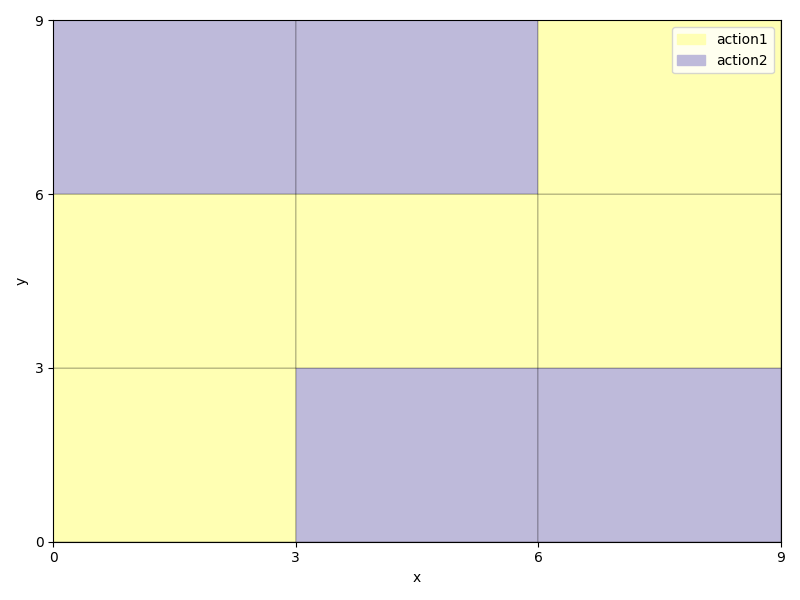
\includegraphics[width=\textwidth]{simpleExamplePartitioning}%
        \caption{}%
        \label{fig:simpleExamplePartitioning}
    \end{subfigure}
    \begin{subfigure}{0.4\textwidth}
      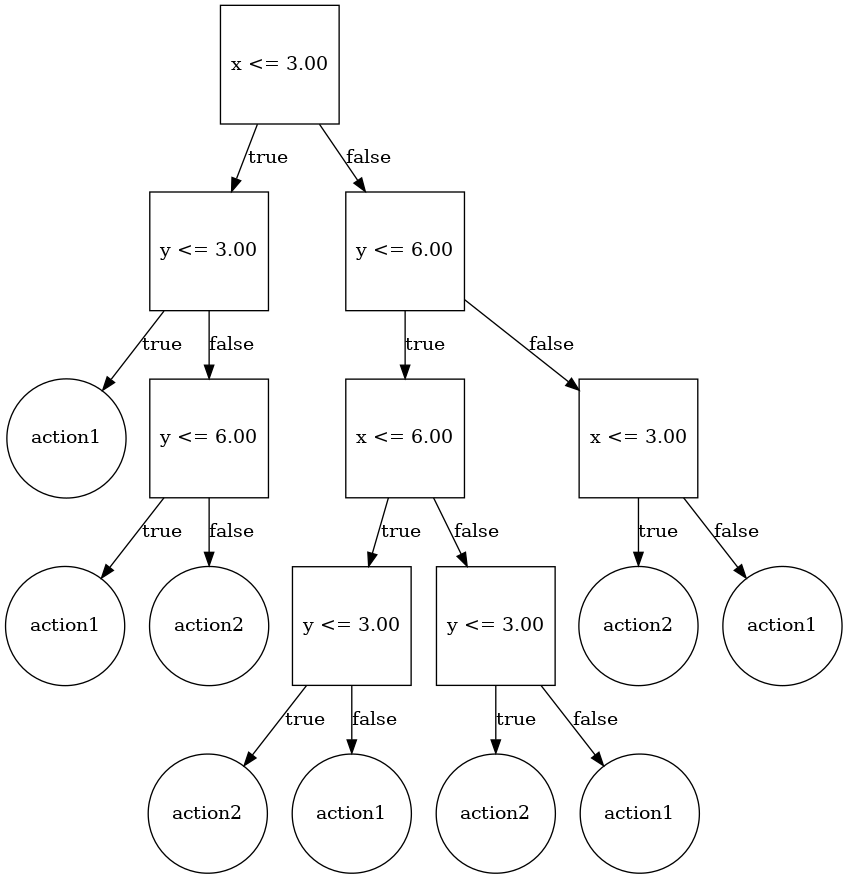
\includegraphics[width=\textwidth]{simpleExampleTree}%
      \caption{}%
      \label{fig:simpleExampleTree}
    \end{subfigure}

  \caption{%
    Two representations of a strategy mapping states to actions. In
    \cref{fig:simpleExamplePartitioning} the strategy is represented as a
    partitioning with colors representing the assigned action. In
    \cref{fig:simpleExampleTree} the strategy is given as a decision
    tree, which also induces the partitioning. For this small example, it is
    obvious to see that an equivalent state-action mapping could be achieved
    with fever regions/leaves.
  }%
  \label{fig:simpleExample}
\end{figure}

However, we can (in this small toy example) easily see that we do not need 9
regions to represent this exact state-action mapping. For example, the two
regions given by $((3,0),(6,3))$ and $((6,0),(9,3))$, respectively, both assign
$action2$ as the optimal action, but this mapping would still be preserved if we
replaced those two regions with a larger one $((3,0),(9,3))$. After a little bit
of inspection, we can actually see here that we could represent the same
state-action mapping with a partitioning consisting of only 5 regions.

This example showcases how discretization techniques can easily end up with
redundancy in the partitioning. This can be very difficult to anticipate before
learning, especially since a very fine-grained discretization is typically
needed for the learning to capture essential information and details for the
strategy. Furthermore, for other learning techniques, such as the online
partitioning refinement scheme of \textsc{UPPAAL Stratego}~\cite{Manfred2019},
regions can be created on-the-fly, not be arranged in a straight grid and/or
vary in size, which can enhance the problem of redundancy.

We propose \textsc{MaxPartitions}, an algorithm that postprocesses a decision
tree inducing a partitioning of a state space in order to minimize the
partitioning by \textit{maximizing} the size of the individual regions (or
partitions). The output of \textsc{MaxPartitions} is a new partitioning, ie.\ a
list of regions with associated actions, which can then be arranged into a new
decision tree.


\subsection{Details of the algorithm}%
\label{sub:maxPartsDescription}

We write $\mathcal{T}_i$ for the (ascendingly) sorted list of bounds on
dimension $i$ in the policy given by the tree $\mathcal{T}$. The first bound in
the list is defined to be negative $\infty$ and the last is positive $\infty$.
By $\mathcal{T}_{i,j}$ we write the $j$th smallest bound on dimension $i$ for
each $j = 1, 2, \ldots, |\mathcal{T}_i|$. This can be precomputed as a matrix in
log-linear time by collecting and sorting the bounds on all branch nodes in
$\mathcal{T}$ and allows accessing $\mathcal{T}_{i,j}$ in constant time.
Further, in a slight abuse of notation, we define $\mathcal{T}_{i,
|\mathcal{T}_i| + 1}$ to be some \textit{sentinel} value representing that we
are outside the boundaries of dimension $i$. Correspondingly, we define a
sentinel action $\alpha$, and we say that $\mathcal{T}(s^p_{\mathcal{T}}) =
\alpha$ if and only if $\exists p_i \in p,\, p_i = |\mathcal{T}_i| + 1$.

Exploiting this notation, let $p$ be a $K$-dimensional vector of integers, such
that $p_i \leq |\mathcal{T}_i| + 1$ for all $i = 1,\ldots,K$, then we can define
a point at an intersection of bounds in $\mathcal{T}$ as $s^{p}_{\mathcal{T}} =
(\mathcal{T}_{1,p_1}, \mathcal{T}_{2,p_2}, \ldots, \mathcal{T}_{K,p_K})$. To
avoid cluttering the notation, we will for the most part omit the subscript
$\mathcal{T}$ on $s^{p}_{\mathcal{T}}$. To make things clear, we will write $s$
to refer to an actual point in the state space of $\mathcal{T}$, ie.\ $s \in
\mathcal{S}$, and we will write $p$ to refer to a vector of integers
representing indicies of bounds in $\mathcal{T}$.

The algorithm (given in pseudo-code in \cref{alg:MaxPartitions}) works
by maintaining a pair $(p^{\min}, p^{\max}$), and iteratively incrementing
$p^{\max}$ in one dimension at a time until a region $\nu = (s^{p^{\min}},
s^{p^{\max}})$ cannot be expanded further. When this happens, the region is
added to a tree $\mathcal{T}_{track}$, which is used to track which areas of the
state space have been covered and to provide new a starting point for each
iteration of the algorithm. Expansion in dimension $i$ is disallowed if one of
the following three \textit{expansion rules} are violated by the expanded region
$\nu'$:

\begin{definition}[Expansion rules]\label{def:expansionRules}
    Let $\nu'$ be a candidate region for a new partitioning derived from
    $\mathcal{A}_{T}$. Then $\nu'$ is valid if it adheres to the following rules:

    \begin{enumerate}
        \item $\nu'$ must have singular mapping in $\mathcal{T}$
        \item $\nu'$ must not intersects with any region already in
            $\mathcal{T}_{track}$
        \item $\nu'$ cannot intersect with a region $\nu_{o}$ in the original
            partitioning, such that the difference $\nu_{o} - \nu'$ cannot be
            described by a single region of the form $(s^{\min}, s^{\min})$
    \end{enumerate}
\end{definition}

\noindent The first two cases are directly related to the definition of the
problem, ie.\ the produced partitioning should respect $\mathcal{T}$ and only
have non-overlapping regions. The third case is required in order to guarantee
that in each iteration the algorithm on average will add \textit{at least} one
region from the original partitioning to the new partitioning. To see this,
consider the visualization in~\cref{fig:expRules3}. The candidate expansion
`cuts' the rightmost region (given by $(3,0)$ and $(4,4)$) in two such that the
remainder would have to be represented by \textit{two} regions --- one given
by $((3,0), (4,2))$ and one given by $((3,3), (4,4))$.

\begin{figure*}[ht]
    \centering
    \begin{subfigure}{0.24\textwidth}
        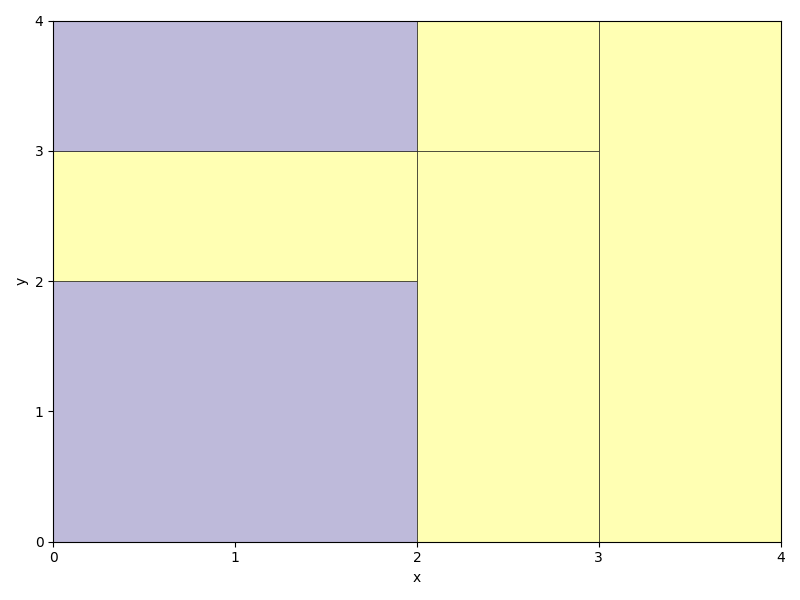
\includegraphics[width=\textwidth]{rules_org}%
        \caption{}%
        \label{fig:expRulesOrg}
    \end{subfigure}
    \begin{subfigure}{0.24\textwidth}
      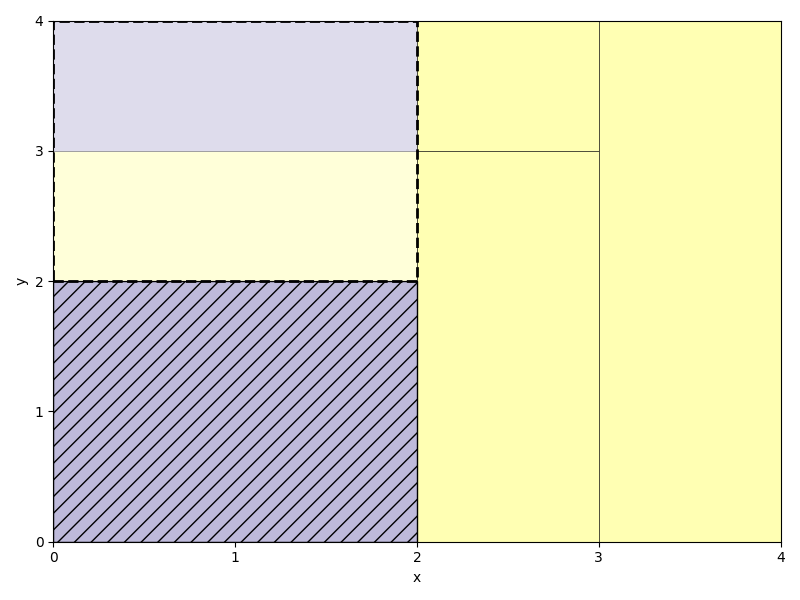
\includegraphics[width=\textwidth]{rule1}%
      \caption{}%
      \label{fig:expRules1}
    \end{subfigure}
    \begin{subfigure}{0.24\textwidth}
      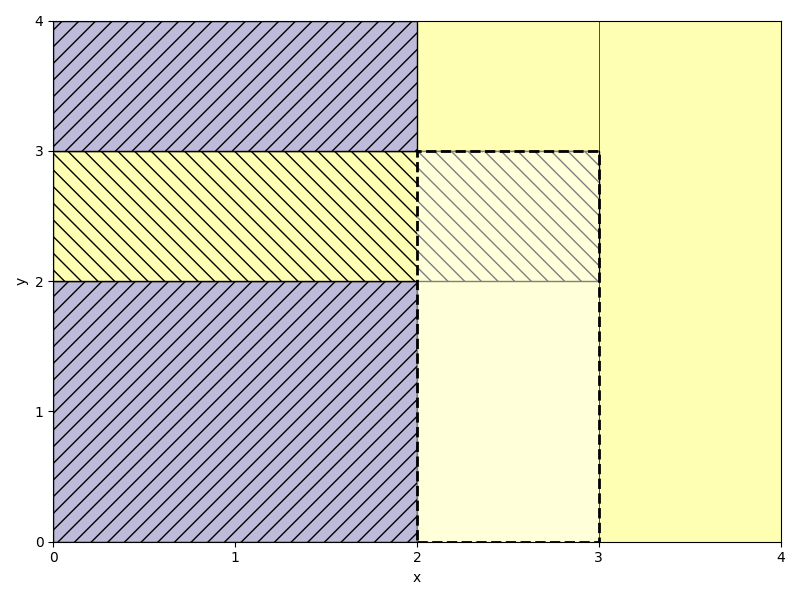
\includegraphics[width=\textwidth]{rule2}%
      \caption{}%
      \label{fig:expRules2}
    \end{subfigure}
    \begin{subfigure}{0.24\textwidth}
      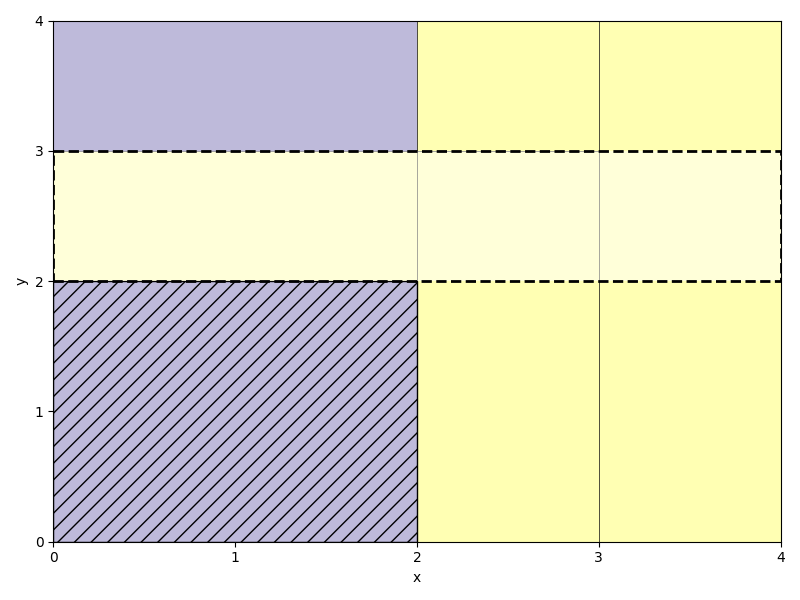
\includegraphics[width=\textwidth]{rule3}%
      \caption{}%
      \label{fig:expRules3}
    \end{subfigure}

  \caption{%
      A visual example of the 3 expansion rules. Striped regions indicate that
      the algorithm has covered this part in a previous iteration, whereas the
      shaded region with a dashed border is a candidate expanded
      region.~\cref{fig:expRulesOrg} shows a potential input partitioning.
      In~\cref{fig:expRules1} the expansion is illegal according to Rule 1,
      since the expanded region contains two different actions
      (colors).~\cref{fig:expRules2} violates Rule 2, since the expanded region
      overlaps with a striped area.~\cref{fig:expRules3} shows a representation
      of the 3rd rule, as the expansion would `cut' the rightmost region in two.
  }%
  \label{fig:expansionRules}
\end{figure*}


How do we determine this expansion? Let $(p^{\min}, p^{\max})$ define (the
remainder of) a region in the original partitioning. We then want to find a
$\Delta_p \in \mathbb{Z}^K$ such that $(p^{\min}, p^{\min} + \Delta_p)$ defines
a region that follows the three expansion rules and such that incrementing in
any one dimension would result in a violation. By definition, a valid value for
$\Delta_p$ is when $\Delta_p = p^{\max} - p^{\min}$, since this would just
produce the original region. We are therefore guaranteed to at least find this
region. This gives rise to the following definition.

% Let $p^{\min}$ be the result of popping the lexicographically smallest element
% of $\mathcal{P}$ (line 4). We can then define $s^{\min} = s^{p^{\min}}$ as the
% `lower left' corner in (or the origin of) a region $\nu = (s^{\min}, s^{\max})$
% where $s^{\max}$ is the point we want to determine, so that $\nu$ is maximized
% and has singular mapping in $\mathcal{T}$. By definition, $s^{\max} =
% s^{p^{\max}}$ satifies the singular mapping requirement for $p^{\max} =
% (p^{\min}_{1} + 1, \ldots, p^{\min}_{K} + 1)$, since no branch node in
% $\mathcal{T}$ splits on a predicate $c$ where $\mathcal{T}_{i,p^{\min}_{i}} < c
% < \mathcal{T}_{i,p^{\min}_{i} + 1}$ for any $i = 1, \ldots, K$.

% Finding a $p^{\max}$ that maximizes the region comes down to finding a vector
% $\Delta_{p} \in \mathbb{Z}^{K}$ so that $p^{\max} = p^{\min} + \Delta_{p}$. The
% definition of $\Delta_{p}$ is given below.

\begin{definition}[The expansion vector $\Delta_p$]\label{def:deltaP}
    Given $p^{\min} \in \mathbb{Z}^{K}$, a decision tree $\mathcal{T}$ over a
    $K$-dimensional space and a decision tree $\mathcal{T}_{track}$ of already
    found regions, $\Delta_{p} \in \mathbb{Z}^{K}$ is a vector such that for
    $p^{\max} = p^{\min} + \Delta_{p}$ the region $\nu =
    (s^{p^{\min}}_{\mathcal{T}}, s^{p^{\max}}_{\mathcal{T}})$ does not violate
    any of the expansion rules in \cref{def:expansionRules} and where
    for any other $\Delta'_p = (\Delta_{p_{1}}, \ldots, \Delta_{p_{i}} + 1,
    \ldots, \Delta_{p_{K}})$ this would not hold.
\end{definition}

\noindent A greedy approach to finding $\Delta_{p}$ starts with $\Delta_{p} =
p^{\max} - p^{\min}$, for some (remainder of a) region $\nu =
(s^{p^{\min}}_{\mathcal{T}}, s^{p^{\max}}_{\mathcal{T}})$. We then iteratively
increment a single dimension chosen non-deterministically untill the invariants
are violated.  Let $\mathbf{\hat{e}}_i$ denote the unit vector parallel to axis
$i$, such that $\Delta_{p} + \mathbf{\hat{e}}_i =
(\Delta_{p_1},\ldots,\Delta_{p_i} + 1,\ldots,\Delta_{p_K})$. At each increment,
we define a candidate region $\nu'$ from $p^{\min}$ and $p^{\max} = p^{\min} +
\Delta_{p}$ and check for singular mapping (Rule 1) and no overlap with regions
in $\mathcal{R}$ (Rule 2). If any of these two do not hold, we mark dimension
$i$ as exhausted, roll back the increment and continue with a new dimension not
marked as exhausted.

If Rule 3 is violated, the algorithm wil initiate an attempt at \textit{healing}
the candidate expansion, by continuing the expansion to the largest bound in
the expansion dimension of any of the broken regions. This way we try to see if
the violation can be overcome by simply expanding more aggressively. However,
care is required to ensure, that we can roll back this extra expansion if it did
not work (or if we inadverdently broke any of the other rules in the process).

When all dimensions have been
exhausted, $\Delta_{p}$ adheres to \cref{def:deltaP}.

\begin{algorithm}[!ht]
    \caption{MaxPartitions}\label{alg:MaxPartitions}

    \begin{algorithmic}[1]
        \Require{%
            $\mathcal{T}$: A binary decision tree over the domain
            $\mathbb{R}^K$ inducing the partitioning $\mathcal{A}_{\mathcal{T}}$
        }
        \State{$\mathcal{T}_{track} \gets$ empty tree}
        \State{$\mathcal{R} \gets \{\}$}

        \While{$\mathcal{T}_{track}$ has unexplored regions}

            \State{%
                $(p^{\min}, p^{\max}) \gets$
                select from unexplored regions
            }

            \State{%
                $\Delta_p \gets p^{\max} - p^{\min}$
            }
            \State{%
                $\Delta'_p \gets \Delta_p$
            }
            \State{%
                \textit{healing} $\gets false$
            }

            \item[]
            \While{%
                not all dimensions have been exhausted
            }

                \If{not \textit{healing}}
                    \State{%
                        $d \gets$ select unexhausted dimension
                    }
                    \State{%
                        $\Delta'_{p} \gets \Delta_{p} + \mathbf{\hat{e}}_d$
                    }
                    % \State{%
                    %     $\Delta_{p_{d}} \gets \Delta_{p_{d}} + 1$
                    % }
                \EndIf%

                \State{%
                    $\nu' \gets (s^{p^{\min}}_{\mathcal{T}}, s^{p^{\min} +
                    \Delta'_p}_{\mathcal{T}})$
                }

                \item[]
                \If{%
                    $\nu'$ violates Rule 1 or 2
                    (\cref{def:expansionRules})
                }
                    \State{%
                        $\Delta'_{p_{d}} \gets
                        \Delta'_{p_{d}} - \mathbf{\hat{e}}_{d}$
                    }
                    \State{mark $d$ as exhausted}
                    \State{$healing \gets false$}
                \item[]

                \ElsIf{%
                    $\nu'$ violates Rule 3 (\cref{def:expansionRules})
                }
                    \State{%
                        $b \gets $ largest bound in $d$ among broken regions
                    }
                    \If{$\Delta'_{p_{d}} < b$}
                        \State{$healing \gets true$}
                        \State{%
                            $\Delta'_{p_{d}} \gets b$ 
                        }
                    \Else%
                        \State{$healing \gets false$}
                        \State{mark $d$ as exhausted}
                    \EndIf%

                    % \State{attempt $healing$ in dimension $d$}

                    % \State{find the smallest expansion value in dimension $d$,
                    %     such that either no rules are violated or Rule 1 or 2 is
                    %     violated. In the first case, use this expansion value
                    %     and continue, in the latter case revert to the last
                    %     legal expansion value and mark dimension $d$ as
                    %     exhausted.
                    % }
                        
                \Else
                    \State{$healing \gets false$}
                    \State{%
                        $\Delta_p \gets \Delta'_p$
                    }
                \EndIf%

            \EndWhile%

            \item[]
            \State{%
                $\nu \gets (s^{p^{\min}}_{\mathcal{T}}, s^{p^{\min} +
                \Delta_p}_{\mathcal{T}})$
            }
            \State{%
                \Call{Put}{$\mathcal{T}_{track},\, \nu$}
            }
            \State{%
                $\mathcal{R} \gets \mathcal{R} \cup \{\nu\}$
            }

        \EndWhile%

        \State{\textbf{return} $\mathcal{R}$}

    \end{algorithmic}

\end{algorithm}



\subsection{Proof of correctness}%
\label{sec:proofCorrectness}

\noindent
Let $\mathcal{B}$ be the output of running \textsc{MaxPartitions} with a
decision tree $\mathcal{T}$ and its induced partitioning
$\mathcal{A}_{\mathcal{T}}$ as input. We want to prove the following properties
of the algorithm:

\paragraph{$\mathcal{B}$ is a partitioning in accordance
with~\cref{def:partitioning}} For this, it is required that for any two regions
$\nu_{i}, \nu_{j} \in \mathcal{B}$ the intersection of $\nu_{i}$ and $\nu_{j}$
must be the empty set and that the union of all regions must consitute the
entire state space. We can see that this must hold because of our use of the
intermediate decision tree $\mathcal{T}_{track}$. Firstly, this is used to honor
the second expansion rule in~\cref{def:expansionRules} which forbids an
expansion that would cause two regions to intersect. Secondly, the algorithm
proceeds excactly for as long as there are unexplored regions in
$\mathcal{T}_{track}$. Since any starting region will either be a region from
$\mathcal{A}_{\mathcal{T}}$ or the remainder of one (because of the third
expansion rule), each iteration will add to $\mathcal{T}_{track}$ a region that
decreases the remainding regions to be explored by at least one, thus
guaranteeing convergence. Therefore, $\mathcal{B}$ will be a partitioning in
accordance with the definition.

\paragraph{$\mathcal{B}$ respects $\mathcal{T}$} The first expansion rule
forbids an expansion that would create a region witout singular mapping in
$\mathcal{T}$. By definition, if all regions in $\mathcal{B}$ as singular
mapping in $\mathcal{T}$ then $\mathcal{B}$ respects $\mathcal{T}$. Since any
starting region is a subset of a region in $\mathcal{A}_{\mathcal{T}}$, which by
definition respects $\mathcal{T}$, neither an expanded region nor a region
returned `as-is' can violate the singular mapping requirement. Therefore,
$\mathcal{B}$ must respect $\mathcal{T}$.\todo{Do we need to prove it with
    relation to our method for finding the expansion vector, ie.\ how we
incrementally do the expansion?}

\paragraph{$|\mathcal{B}| \leq |\mathcal{A}_{\mathcal{T}}|$} At each iteration,
the algorithm starts with a region $\nu$ that is a subset of a region in
$\nu_{o} \in \mathcal{A}_{\mathcal{T}}$. The algorithm attempts to expand the region and
when that is no longer possible, it is added to the output partitioning
$\mathcal{B}$. For $\mathcal{B}$ to be larger than $\mathcal{A}_{\mathcal{T}}$
would therefore require, that at least two starting regions $\nu_{i},
\nu_{j}$ in separate iterations of the algorithm are disjoint subsets of the
same region in $\mathcal{A}_{\mathcal{T}}$. When the algorithm starts, this
cannot be the case, since any starting region will be identical to a region from
the input partitioning. Now, the third expansion rule prohibits an expansion, if
for some region $\nu_{i} \in \mathcal{A}_{\mathcal{T}}$ the expanded region
$\nu'$ would cause $\nu_{i} - \nu'$ to be non-convex, ie.\ not representable on
the form $(s^{\min}, s^{\max})$. This means, that whenever a region $\nu$ is
selected as a starting region, either $\nu$ will be identical to a region in
$\nu_{o} \in \mathcal{A}_{\mathcal{T}}$ or it will be the only remainding subset
of $\nu_{o}$ not covered by any of the expanded regions already in
$\mathcal{B}$. Therefore, under no circumstances can there be added more regions
to $\mathcal{B}$ than the number of regions in $\mathcal{A}_{\mathcal{T}}$ and
as such we can guarantee that $|\mathcal{B}| \leq |\mathcal{A}_{\mathcal{T}}|$.

% \subsection{Complexity}%
% \label{sec:complexity}

\subsection{From regions to decision tree}%
\label{sub:regionsToDT}

The output of the \textsc{MaxPartitions} algorithm is a list of regions with
associated actions. For this to be of any use, we need to construct a new
decision tree to represent these state-action pairs. To this goal, we face the
issue that it is not given (and in fact, very unlikely) that the suggested
partitioning can be perfectly represented by a decision tree, as this would
require the existence of enough `clean splits' (ie.\ predicates on some variable
that perfectly divides the regions into two sets with an empty intersection) to
arrange the entire set of regions.

For classical decision tree construction algorithms, such as CART~\cite{?},
ID3~\cite{?} and C4.5~\cite{?}, the input is data points that need to be
properly arranged by creating branches according to some splitting criteria
(typically the gini index or entropy). In our case, the data is already arranged
in regions specifying only one label (action) per region, and we want these
regions to be preserved as well as possible as leaves in the tree. We therefore
suggest the following method for choosing a splitting criteria.

Let $\mathbf{R}$ be a list of regions. For notational purposes, we will in the
following refer to $s^{\min}$ and $s^{\max}$ of a region $\nu$ by $\nu_{\min}$
and $\nu_{\max}$ respectively, and to the value of a specific dimension $i$ in
one such boundary point as $\nu_{\min, i}$ or $\nu_{\max,i}$.  Given a list of
regions $\mathbf{R}$, our goal is to find a predicate function $\rho(x) = x_{i}
\leq c$ with $c \in \mathbb{R}$ that, according to some heuristic, splits
$\mathbf{R}$ into two subsets $\mathbf{R}_{low}$ and $\mathbf{R}_{high}$ such
that $\mathbf{R}_{low} = \{ \nu \in \mathbf{R} \mid \rho(\nu_{\min}) = false \}$
and $\mathbf{R}_{high} = \{ \nu \in \mathbf{R} \mid \rho(\nu_{\max}) = true \}$.
Additionally, we require that $\mathbf{R}_{low}$ and $\mathbf{R}_{high}$ are
disjoint, meaning that if for some region $\nu$ it holds that $\rho(\nu_{\min})
= true$ and $\rho(\nu_{\max}) = false$, then $\nu$ must be split so we get two
new regions $\nu', \nu''$ where $\nu' \in \mathbf{R}_{low}$ and $\nu'' \in
\mathbf{R}_{high}$. While $\mathbf{R}$ is greater than one, we create a branch
node from the obtained predicate function and recursively repeat the procedure
for $\mathbf{R}_{low}$ and $\mathbf{R}_{high}$. If $\mathbf{R}$ only contains
one region, we create a leaf node and stop the recursion.

% We iteratively create a branch node that splits $\mathbf{R}$ into two,
% $\mathbf{R}_{low}$ and $\mathbf{R}_{high}$, based on a predicate function
% $\rho(x) = x_i \le c$ with $c \in \mathbb{R}$ so that $\mathbf{R}_{low} = \{ \nu
% \in \mathbf{R} \mid \rho(\nu_{\min}) \text{~is True} \}$ and $\mathbf{R}_{high}
% = \{ \nu \in \mathbf{R} \mid \rho(\nu_{\max}) \text{~is False} \}$. When the
% list only contains a single element $\nu$, we create a leaf node with action
% $a_{\nu}$ and return.

% this figure belongs to the section on "Repeated application", but it shows up
% weird if I put it there
\begin{figure*}[ht]
    \centering
    \begin{subfigure}{0.32\textwidth}
        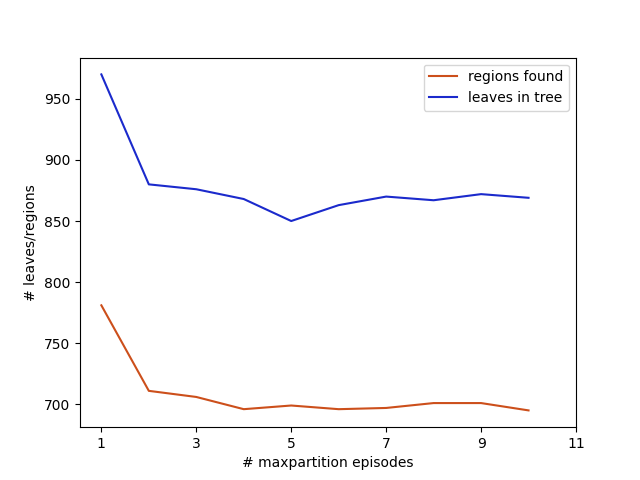
\includegraphics[width=\textwidth]{iterMpBB}%
        \caption{Bouncing Ball}%
        \label{fig:iterativeMaxpartsBB}
    \end{subfigure}
    \begin{subfigure}{0.32\textwidth}
        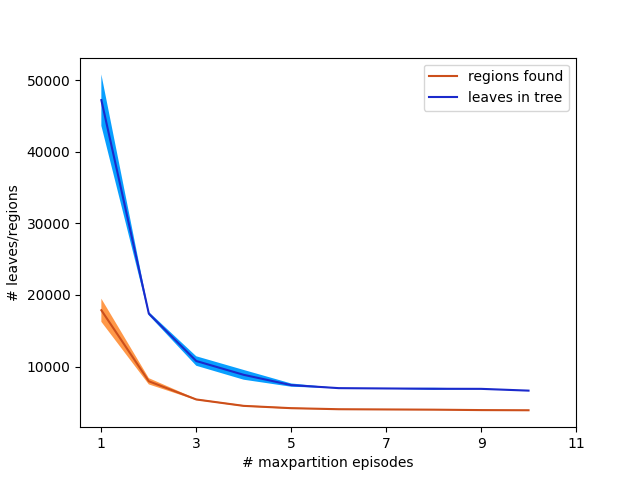
\includegraphics[width=\textwidth]{iterMpCP}%
        \caption{Cartpole}%
        \label{fig:iterativeMaxpartsCP}
    \end{subfigure}
    \begin{subfigure}{0.32\textwidth}
        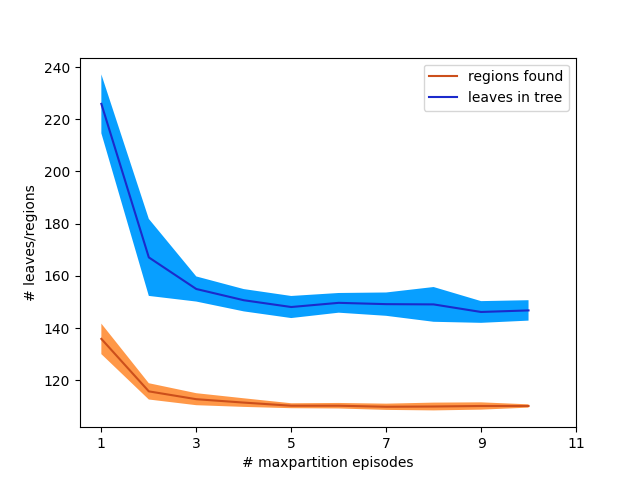
\includegraphics[width=\textwidth]{iterMpTL}%
        \caption{Traffic Light}%
        \label{fig:iterativeMaxpartsTL}
    \end{subfigure}
    \caption{%
        Progression of repeated application of \textsc{MaxPartitions} on
        different models. Each graph starts after 1 minimization step.
    }\label{fig:iterativeMaxparts}
\end{figure*}

We define a heuristic for choosing $\rho$ that balances trying to create a
balanced tree with trying to maintain the structure of the input regions.
Ideally, we want to split $\mathbf{R}$ in two equally sized subsets and in a way
that no region would have to be split, ie.\ we would like
$|\mathbf{R}_{low}| + |\mathbf{R}_{high}| = |\mathbf{R}|$. For this we define an
impurity measure $I(\mathbf{R},\rho)$ that penalises the
difference in size between $\mathbf{R}_{low}$ and $\mathbf{R}_{high}$ and the
number of regions split. Let $abs(a)$ be the absolute value of
$a$ and let $s = abs(|\mathbf{R}| - (|\mathbf{R}_{low}| + |\mathbf{R}_{high}|))$
be the number of split regions, then

\[
    I(\mathbf{R}, \rho)  = abs(|\mathbf{R}_{low}| -
    |\mathbf{R}_{high}|) + s
\]

To calculate this impurity, we can sort the list of regions according to the
dimension in which we want to try and split the list. Let $\mathbf{R}_i = \{
\nu^1, \nu^2, \ldots, \nu^n \}$ be the list sorted according to the $i$th
dimension so that for all $\nu^j, \nu^{j+1} \in \mathbf{R}_{i}$ it holds that
$\nu^{j}_{\max,i} \le \nu^{j+1}_{\max,i}$. If we then let $\rho(x) = x_i \le c$
with $c = \nu^{j}_{\max,i}$ we have $|\mathbf{R}_{low}| = j$ and
|$\mathbf{R}_{high}| = n - j$. For determining the number of split regions, we
simply need to count the number of regions $\nu^{j+m}$ for $m = 1, 2, \ldots,
n-j$ whose lower bound is less than our predicate bound $c$.

% , since for these regions
% will appear both in $\mathbf{R}_{low}$ and in $\mathbf{R}_{high}$ (because our
% sorting ensures that for all $\nu^{j},\nu^{j+m}$ it holds that $\nu^{j}_{\max,i}
% \le \nu^{j+m}_{\max,i}$).

Now we can write our impurity measure in terms of these quantities:

\[
    I(\mathbf{R}_{i}, \rho)
    % I(\mathbf{R}_{low}, \mathbf{R}_{high})
    = abs(j - (n - j)) +
    \sum^{n}_{m=1} \mathbbm{1}(\rho(\nu^{j+m}_{\min}))
\]

% \noindent
% where $\mathbbm{1}$ is the indicator function, $j = |\mathbf{R}_{low}|$, $n =
% |\mathbf{R}_{low}| + |\mathbf{R}_{high}|$ and $\rho$ is the predicate function
% that has been used to split $\mathbf{R}_{low}$ and $\mathbf{R}_{high}$ and which
% takes the form $\rho(x) = x_{i} \leq c$ with $c = \nu^{j}_{\max, i}$. 

\noindent
where $\mathbbm{1}$ is the indicator function, $\rho$ is a predicate function
of the form $\rho(x) = x_{i} \leq c$ with $c = \nu^{j}_{\max, i}$,
$\mathbf{R}_{i}$ is the set of regions to be split sorted in non-decreasing
order according to $\nu_{\max,i}$ for all $\nu \in \mathbf{R}_{i}$, $n$ is the
number of regions in $\mathbf{R}_{i}$ and $j$ is the largest index such that
$\rho(\nu^{j}_{\max})$ evaluates to true.

Finding the best split, ie.\ the one that minimizes the impurity, is a $O(Kn^2)$
operation, as it requires checking all $K \times n$ possible splitting criterias
and evaluating the impurity function for each of them in time propertional to
$n$. In this work, we have not attempted to find a faster implementation as we
found that the size of the output partitioning from \textsc{MaxPartitions} did
not cause performance issues.

\subsection{Iterative application}%
\label{sub:iterativeApp}

Since \textsc{MaxPartitions} cannot guarantee optimal minimization but selects
its expansion dimensions non-deterministically, we can achieve better
minimization by repeated application of the algorithm. The pipeline is as
follows:

\begin{center}
    \begin{tikzpicture}[every node/.style={scale=0.8}]
        \node (input)                       {$\mathcal{T}$};
        \node (output)  [below=of input]    {$\mathcal{B}$};
        \node (tree)    [below=of output]   {$\mathcal{T}'$};

        \draw [arrow] (input)  -- node[anchor=west] {minimize with \textsc{MaxPartitions}} (output);
        \draw [arrow] (output) -- node[anchor=west] {convert partitioning to new tree} (tree);
        \draw [arrow] (tree)   to [bend left=45] node[anchor=east] {use tree as new input} (input);
    \end{tikzpicture}
\end{center}

We repeat this process untill no improvements in seen in (the size of) neither
the output partitioning nor the new tree. We show experimentally that the major
minimization is achieved in the first step, and that the size of the
output typically stabilizes in less than 10 iterations. Because the most
significant reduction is achieved in the first application, the following
repetitions are fairly inexpensive in terms of running time.

Figure~\cref{fig:iterativeMaxparts} shows the progression over several
iterations for three different examples. Note that the precise size of both the
number of regions in the output partitioning and the size of the constructed
tree continues to fluctuate, since the non-deterministic choices in the
algorithm prevents convergence to a fixed point.

\section{VIPER}%
\label{sec:viper}

\textcolor {orange} {\lipsum[2]}
